\documentclass[a4]{article}

% PAQUETES %%%%%%%%%%%%%%%%%%%%%%%%%%%%%%%%%%%%%%%%%%%%%%%%%%%%%%%%%%%%%%%%%%%%%
\usepackage[utf8]{inputenc}
\usepackage{framed} % Para crear cuadros alrededor del texto
\usepackage{makecell}
\usepackage[english]{babel}
%
\usepackage[fixlanguage]{babelbib}
    \bibliographystyle{IEEEtran}

\usepackage{url}

%!TEX encoding = UTF-8 Unicode
% !TEX spellcheck = es

\setlength{\textwidth}{6.5 in}
\setlength{\textheight}{8.5 in}
\setlength{\headsep}{0.5 in}

\usepackage{multirow, array} % para las tablas
\usepackage{float} % para usar [H]
\usepackage{charter}

\usepackage[breaklinks=true]{hyperref}

%
% ADD PACKAGES here:
%

\usepackage[utf8]{inputenc}
\usepackage{amsmath,longtable,siunitx, float, graphicx, dcolumn, bm, fancyhdr, authblk, subcaption, caption, hyperref, multicol, setspace}

\usepackage{bbding}
\usepackage{amssymb}
\usepackage[rightcaption]{sidecap}
%\usepackage{textcomp}

\usepackage[hmarginratio=1:1, top=32mm, columnsep=20pt, headsep=\dimexpr20mm, margin=0.7in, top=1in ]{geometry}

\usepackage{booktabs}
\usepackage{multirow}

\usepackage{algorithm}
\usepackage{enumitem}
\usepackage{tabularx}
\usepackage[noend]{algpseudocode}
\usepackage{xcolor}

\usepackage{tikz}
\usetikzlibrary{shapes.geometric, arrows.meta, positioning}

% ----------- global styles -----------
\tikzset{
  font=\scriptsize,                      % tiny text everywhere
  every node/.style       = {transform shape},   % respect scale
  startstop/.style        = {ellipse, draw, fill=blue!10,
                             inner sep=1pt, minimum width=13mm},
  process/.style          = {rectangle, draw, fill=orange!15,
                             text width=26mm, inner sep=2pt, align=center},
  decision/.style         = {diamond, draw, fill=green!15, aspect=2.3,
                             text width=20mm, inner sep=1pt, align=center},
  arrow/.style            = {->, >=Stealth, shorten >=1pt, shorten <=1pt}
}

\newcommand{\TODO}{\textbf{\textcolor{red}{TODO}}}

\renewcommand{\algorithmicrequire}{\textbf{Input:}}
\renewcommand{\algorithmicensure}{\textbf{Output:}}

\lhead{\includegraphics[scale=0.4]{CETC.png}}
\rhead{\includegraphics[scale=0.025]{Cornell-University-Logo.png}}

\newtheorem{theo}{Theorem}
\newenvironment{theorem}
  {\begin{mdframed}\begin{theo}}
  {\end{theo}\end{mdframed}}
  
\newtheorem{prop}{Proposición}
\newenvironment{proposition}
  {\begin{mdframed}\begin{prop}}
  {\end{prop}\end{mdframed}}

\newtheorem{lem}{Lema}
\newenvironment{lema}
  {\begin{mdframed}\begin{lem}}
  {\end{lem}\end{mdframed}}
  
\newtheorem{defi}{Definition}
\newenvironment{definition}
  {\begin{mdframed}\begin{def}}
  {\end{def}\end{mdframed}}
  
\newtheorem{proof}{Proof}
\newtheorem{remark}{Remark}

\usepackage[numbers]{natbib}
\renewcommand{\thesection}{\Roman{section}}
%\setlength{\parskip}{\baselineskip}%

\begin{document}

\thispagestyle{fancy}

\begin{center}
    \textbf{\large Orbit Odyssey - Computer Vision} \\
    {Field Definition}
    
    \vspace{0.7em}

    David Alejandro Fuquen \\

    {\small \today}

\end{center}

\section*{Playing Field Definition}

\subsection*{Summary}
This part of Phase 1 defines all the structure, positions, conditions and specifications for the playing field. This is the first part of the competition manual. For this case, we will consider the partition of the original field will be taken away. 


\section*{Field dimensions, boundaries and markings}
We will use the same dimensions and boundaries as the original Space Odyssey. The same 4x8 field will be used, without the inner field partition. 

The playing field is a rectangular arena enclosed by low-profile PVC pipe barriers on all four sides.

\begin{table}[H]
\centering
\begin{tabular}{ll}
\toprule
\textbf{Property} & \textbf{Value} \\
\midrule
Total length (X-axis) & 254.00 cm (100 in) \\
Total width (Y-axis) & 142.24 cm (56 in) \\
Total floor area & 3.61 m\textsuperscript{2} \\
Perimeter walls & Low-profile PVC pipe barriers \\
Corner zones & 30.48 $\times$ 30.48 cm (12 $\times$ 12 in) at each corner \\
Partition & \textbf{Removed} \\
\bottomrule
\end{tabular}
\caption{Field dimensions and boundaries.}
\end{table}

The coordinate system places the origin $(0, 0)$ at the bottom-left corner of the field. The X-axis runs left to right (0 to 254 cm) and the Y-axis runs bottom to top (0 to 142.24 cm). Four corner zones of 12 $\times$ 12 in are marked at each corner and serve as robot starting areas --- no objects may be placed inside these zones.

\begin{figure}[H]
\centering
\begin{tikzpicture}
  \begin{scope}[scale=0.055]
    \draw[thick] (0,0) rectangle (254, 142.24);
    \draw[dashed, blue!60] (0,0) rectangle (30.48, 30.48);
    \draw[dashed, blue!60] (254-30.48,0) rectangle (254, 30.48);
    \draw[dashed, blue!60] (0,142.24-30.48) rectangle (30.48, 142.24);
    \draw[dashed, blue!60] (254-30.48,142.24-30.48) rectangle (254, 142.24);
    \filldraw[red!70!black] (63.50, 35.56) circle (6);
    \filldraw[red!70!black] (190.50, 35.56) circle (6);
    \filldraw[red!70!black] (127.00, 71.12) circle (6);
    \filldraw[red!70!black] (63.50, 106.68) circle (6);
    \filldraw[red!70!black] (190.50, 106.68) circle (6);
    \draw[dashed, gray!50] (63.50,35.56) -- (127.00,71.12) -- (190.50,35.56);
    \draw[dashed, gray!50] (63.50,106.68) -- (127.00,71.12) -- (190.50,106.68);
    \draw[dashed, gray!50] (63.50,35.56) -- (63.50,106.68);
    \draw[dashed, gray!50] (190.50,35.56) -- (190.50,106.68);
    \draw[<->, >=Stealth] (0,-12) -- (254,-12);
    \draw[<->, >=Stealth] (-12,0) -- (-12,142.24);
  \end{scope}
  \node[font=\footnotesize\bfseries, anchor=north] at (3.49,1.63) {\textsf{P1}};
  \node[font=\footnotesize\bfseries, anchor=north] at (10.48,1.63) {\textsf{P2}};
  \node[font=\footnotesize\bfseries, anchor=west] at (7.35,3.91) {\textsf{P3}};
  \node[font=\footnotesize\bfseries, anchor=south] at (3.49,6.20) {\textsf{P4}};
  \node[font=\footnotesize\bfseries, anchor=south] at (10.48,6.20) {\textsf{P5}};
  \node[blue!70, font=\scriptsize] at (0.84,0.84) {LRZ};
  \node[blue!70, font=\scriptsize] at (13.13,0.84) {LRZ};
  \node[blue!70, font=\scriptsize] at (0.84,6.98) {LRZ};
  \node[blue!70, font=\scriptsize] at (13.13,6.98) {LRZ};
  \node[font=\footnotesize] at (6.99,-1.10) {254 cm (100 in)};
  \node[font=\footnotesize, rotate=90] at (-1.21,3.91) {142.24 cm (56 in)};
  \node[font=\scriptsize, anchor=north east] at (-0.11,-0.11) {$(0,0)$};
\end{tikzpicture}
\caption{Layout NP\_5 --- diamond pattern with center point (no partition).}
\end{figure}

//TODO (David): Add an image with the field. DON'T DO THIS, I'll do it myself.

\section*{Robot starting zone and placement rules}
The Robot will start in any of the two corners known as \textit{Low Rubble Zone} in the original orbit Odyssey. So long the robot is within the boundaries of that corner, the team may decide where the robots points to. Ideally, this will be the only human-made decision of the challenge, the only part in which the team has any kind of decision-making ablities. 

\section*{Object quantity, placement templates, and clearance constraints}
\subsection*{Object count and class breakdown}
This layout uses \textbf{5 objects}: 1 Rocket (contact) + 2 Tires (avoid) + 2 Tin Cans (avoid). Each object has an approximate radius of 6 cm for clearance calculations. The objects are arranged in a \textbf{diamond pattern with a center point}, providing symmetric coverage of the field.

\subsection*{Object positions}

\begin{table}[H]
\centering
\begin{tabular}{clccccl}
\toprule
\textbf{ID} & \textbf{Location} & \textbf{X (in)} & \textbf{Y (in)} & \textbf{X (cm)} & \textbf{Y (cm)} \\
\midrule
P1 & Bottom-left quadrant & 25 & 14 & 63.50 & 35.56 \\
P2 & Bottom-right quadrant & 75 & 14 & 190.50 & 35.56 \\
P3 & Dead center & 50 & 28 & 127.00 & 71.12 \\
P4 & Top-left quadrant & 25 & 42 & 63.50 & 106.68 \\
P5 & Top-right quadrant & 75 & 42 & 190.50 & 106.68 \\
\bottomrule
\end{tabular}
\caption{Object positions --- Layout NP\_5.}
\end{table}

\subsection*{Clearance verification}

\textbf{Minimum clearances:} object center to wall $\geq$ 20 cm, object center to object center $\geq$ 35 cm, objects must be outside all corner zones.

\begin{table}[H]
\centering
\begin{tabular}{ccccccc}
\toprule
\textbf{ID} & \textbf{Left wall} & \textbf{Right wall} & \textbf{Bottom wall} & \textbf{Top wall} & \textbf{Min wall} & \textbf{Nearest obj.} \\
\midrule
P1 & 63.5 & 190.5 & 35.6 & 106.7 & 35.6 \checkmark & 71.1 (P4) \checkmark \\
P2 & 190.5 & 63.5 & 35.6 & 106.7 & 35.6 \checkmark & 71.1 (P5) \checkmark \\
P3 & 127.0 & 127.0 & 71.1 & 71.1 & 71.1 \checkmark & 72.8 (P1) \checkmark \\
P4 & 63.5 & 190.5 & 106.7 & 35.6 & 35.6 \checkmark & 71.1 (P1) \checkmark \\
P5 & 190.5 & 63.5 & 106.7 & 35.6 & 35.6 \checkmark & 71.1 (P2) \checkmark \\
\bottomrule
\end{tabular}
\caption{Clearance verification (all values in cm).}
\end{table}

\subsection*{Distance from each corner to each object (cm)}

\begin{table}[H]
\centering
\begin{tabular}{lccccc}
\toprule
\textbf{Corner} & \textbf{P1} & \textbf{P2} & \textbf{P3} & \textbf{P4} & \textbf{P5} \\
\midrule
Bottom-Left & \textbf{52} & 176 & 125 & 103 & 198 \\
Bottom-Right & 176 & \textbf{52} & 125 & 198 & 103 \\
Top-Left & 103 & 198 & 125 & \textbf{52} & 176 \\
Top-Right & 198 & 103 & 125 & 176 & \textbf{52} \\
\bottomrule
\end{tabular}
\caption{Distance from each corner zone center to each object position.}
\end{table}

The layout is perfectly symmetric: every corner has the same distance profile (one object at $\sim$52 cm, one at $\sim$103 cm, center at $\sim$125 cm, and two far objects at $\sim$176 and $\sim$198 cm). No corner has an advantage.

\subsection*{Suggested class rotation templates}

Positions are physically fixed for the entire event. Between heats, the referee changes which class is assigned to which position.

\begin{table}[H]
\centering
\begin{tabular}{lccccc}
\toprule
\textbf{Template} & \textbf{P1} & \textbf{P2} & \textbf{P3} & \textbf{P4} & \textbf{P5} \\
\midrule
A & Rocket & Tire & Tin Can & Tire & Tin Can \\
B & Tin Can & Rocket & Tire & Tin Can & Tire \\
C & Tire & Tin Can & Rocket & Tin Can & Tire \\
D & Tire & Tin Can & Tin Can & Rocket & Tire \\
\bottomrule
\end{tabular}
\caption{Class rotation templates.}
\end{table}






\end{document}
